\documentclass{standalone}
\usepackage{pgfplots}
\usepackage{sansmath}
\pgfplotsset{compat=1.16}
\definecolor{bg}{HTML}{D8D8D8}
\definecolor{Display}{HTML}{1F77B4}
\definecolor{LowerExp}{HTML}{FF7F0E}
\definecolor{dtoa}{HTML}{2CA02C}
\definecolor{ryu}{HTML}{D62728}
\definecolor{teju}{HTML}{9467BD}
\definecolor{zmij}{HTML}{9C564B}
\tikzset{
  on layer/.code={
    \pgfonlayer{#1}\begingroup
    \aftergroup\endpgfonlayer
    \aftergroup\endgroup
  },
}
\pgfplotsset{
  every axis/.append style={
    x=12pt,
    height=3.5in,
    xmin=0.5,
    ymin=0,
    ymax=149,
    xtick pos=bottom,
    xtick distance=5,
    xticklabel shift=-1pt,
    tick label style={font=\sansmath\sffamily},
    every axis label={font=\sansmath\sffamily},
    label style={font=\sansmath\sffamily},
    ymajorgrids=true,
    major grid style={line width=0.8pt,draw=gray!55},
    axis background/.style={fill=bg},
  },
  every axis plot/.append style={
    line width=0.8pt,
    mark=*,
    forget plot,
  },
  area legend/.style={
    legend image code/.code={
      \draw[#1] (0pt,0.3pt) rectangle (0.9em,1.4ex);
    },
  },
  highlight/.style={
    preaction={
      on layer=pre main,
      line width=6pt,
      opacity=0.5,
      line cap=round,
      line join=round,
      yellow,
    },
  },
}
\begin{document}
\pagecolor{white}
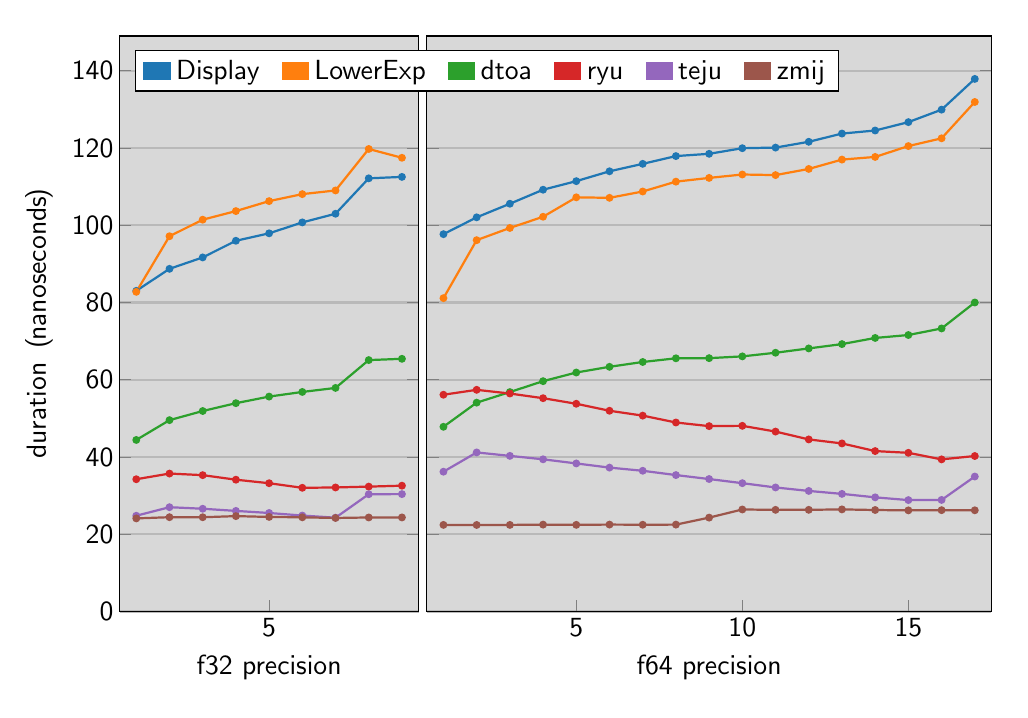
\begin{tikzpicture}[
  every mark/.append style={mark size=1pt},
]
\begin{axis}[
  name=f32,
  xmax=9.5,
  xlabel={f32 precision},
  ylabel={duration\enskip(\kern-1pt nanoseconds\kern-1pt)},
  yticklabel shift=-1.25pt,
  set layers,
  legend style={
    anchor=north west,
    at={(0.05,0.975)},
    font=\sansmath\sffamily,
    /tikz/every even column/.append style={column sep=6pt},
    nodes={anchor=base, inner ysep=0.5pt},
    execute at begin node={\rule{0pt}{8pt}},
  },
  legend cell align=left,
  legend columns=-1,
]
  \addlegendentry{Display}
  \addlegendimage{color=Display, fill, area legend}
  \addplot[color=Display] coordinates {
    (1, 83.01)
    (2, 88.71)
    (3, 91.66)
    (4, 95.97)
    (5, 97.90)
    (6, 100.73)
    (7, 102.97)
    (8, 112.14)
    (9, 112.51)
  };
  \addlegendentry{LowerExp}
  \addlegendimage{color=LowerExp, fill, area legend}
  \addplot[color=LowerExp] coordinates {
    (1, 82.75)
    (2, 97.15)
    (3, 101.43)
    (4, 103.66)
    (5, 106.24)
    (6, 108.05)
    (7, 109.00)
    (8, 119.74)
    (9, 117.46)
  };
  \addlegendentry{dtoa}
  \addlegendimage{color=dtoa, fill, area legend}
  \addplot[color=dtoa] coordinates {
    (1, 44.40)
    (2, 49.53)
    (3, 51.89)
    (4, 53.92)
    (5, 55.63)
    (6, 56.83)
    (7, 57.87)
    (8, 65.08)
    (9, 65.41)
  };
  \addlegendentry{ryu}
  \addlegendimage{color=ryu, fill, area legend}
  \addplot[color=ryu] coordinates {
    (1, 34.23)
    (2, 35.70)
    (3, 35.29)
    (4, 34.11)
    (5, 33.20)
    (6, 32.01)
    (7, 32.10)
    (8, 32.32)
    (9, 32.56)
  };
  \addlegendentry{teju}
  \addlegendimage{color=teju, fill, area legend}
  \addplot[color=teju] coordinates {
    (1, 24.78)
    (2, 26.99)
    (3, 26.59)
    (4, 26.03)
    (5, 25.49)
    (6, 24.83)
    (7, 24.27)
    (8, 30.35)
    (9, 30.38)
  };
  \addlegendentry{zmij}
  \addlegendimage{color=zmij, fill, area legend}
  \addplot[color=zmij] coordinates {
    (1, 24.09)
    (2, 24.40)
    (3, 24.39)
    (4, 24.68)
    (5, 24.47)
    (6, 24.37)
    (7, 24.20)
    (8, 24.33)
    (9, 24.34)
  };
\end{axis}
\begin{axis}[
  name=f64,
  at=(f32.east),
  anchor=west,
  xshift=3pt,
  xmax=17.5,
  xlabel={f64 precision},
  yticklabel=\empty,
  set layers,
]
  \addplot[color=Display] coordinates {
    (1, 97.68)
    (2, 102.04)
    (3, 105.56)
    (4, 109.19)
    (5, 111.41)
    (6, 113.96)
    (7, 115.89)
    (8, 117.90)
    (9, 118.49)
    (10, 119.94)
    (11, 120.10)
    (12, 121.60)
    (13, 123.73)
    (14, 124.52)
    (15, 126.69)
    (16, 129.92)
    (17, 137.88)
  };
  \addplot[color=LowerExp] coordinates {
    (1, 81.12)
    (2, 96.13)
    (3, 99.29)
    (4, 102.19)
    (5, 107.22)
    (6, 107.09)
    (7, 108.73)
    (8, 111.28)
    (9, 112.25)
    (10, 113.13)
    (11, 112.98)
    (12, 114.57)
    (13, 116.99)
    (14, 117.68)
    (15, 120.49)
    (16, 122.50)
    (17, 131.91)
  };
  \addplot[color=dtoa] coordinates {
    (1, 47.81)
    (2, 54.06)
    (3, 56.80)
    (4, 59.62)
    (5, 61.86)
    (6, 63.34)
    (7, 64.59)
    (8, 65.54)
    (9, 65.58)
    (10, 66.04)
    (11, 66.98)
    (12, 68.10)
    (13, 69.22)
    (14, 70.81)
    (15, 71.57)
    (16, 73.27)
    (17, 79.99)
  };
  \addplot[color=ryu] coordinates {
    (1, 56.11)
    (2, 57.38)
    (3, 56.42)
    (4, 55.21)
    (5, 53.77)
    (6, 51.96)
    (7, 50.70)
    (8, 48.92)
    (9, 47.98)
    (10, 48.06)
    (11, 46.57)
    (12, 44.54)
    (13, 43.50)
    (14, 41.52)
    (15, 41.07)
    (16, 39.37)
    (17, 40.24)
  };
  \addplot[color=teju] coordinates {
    (1, 36.18)
    (2, 41.17)
    (3, 40.28)
    (4, 39.39)
    (5, 38.32)
    (6, 37.24)
    (7, 36.42)
    (8, 35.31)
    (9, 34.28)
    (10, 33.21)
    (11, 32.10)
    (12, 31.20)
    (13, 30.44)
    (14, 29.54)
    (15, 28.83)
    (16, 28.87)
    (17, 34.93)
  };
  \addplot[color=zmij] coordinates {
    (1, 22.41)
    (2, 22.39)
    (3, 22.40)
    (4, 22.48)
    (5, 22.42)
    (6, 22.49)
    (7, 22.45)
    (8, 22.48)
    (9, 24.29)
    (10, 26.40)
    (11, 26.30)
    (12, 26.31)
    (13, 26.42)
    (14, 26.26)
    (15, 26.17)
    (16, 26.22)
    (17, 26.19)
  };
  \legend{};
\end{axis}
\pgfresetboundingbox\path
  (f32.south west) -- ++(-0.46in,-0.39in)
  rectangle (f64.north east) -- ++(6pt,3pt);
\end{tikzpicture}
\end{document}
